\chapter{\ifenglish Background Knowledge and Theory\else ทฤษฎีที่เกี่ยวข้อง\fi}

การทำโครงงาน เริ่มต้นด้วยการศึกษาค้นคว้า ทฤษฎีที่เกี่ยวข้อง หรือ งานวิจัย/โครงงาน ที่เคยมีผู้นำเสนอไว้แล้ว ซึ่งเนื้อหาในบทนี้ก็จะเกี่ยวกับการอธิบายถึงสิ่งที่เกี่ยวข้องกับโครงงาน เพื่อให้ผู้อ่านเข้าใจเนื้อหาในบทถัดๆ ไปได้ง่ายขึ้น

\section{Brief Rules of Root} \label{brief-rules-of-root}
Root is a 2-4 player turn-based game, where you play as one of the four factions, fighting against other factions to be the ruler of woodland.

The rule is simple: the player who gets 30 victory points or plays and completes the dominance card (the card that change the endgame winning condition) first wins. The players play on the map of Woodland (Fig 2.1), which contains 12 clearings, each with different suits and different number of slots for building. There are also paths that connect those clearings for moving warriors from one to another clearing.

\begin{figure}
  \begin{center}
    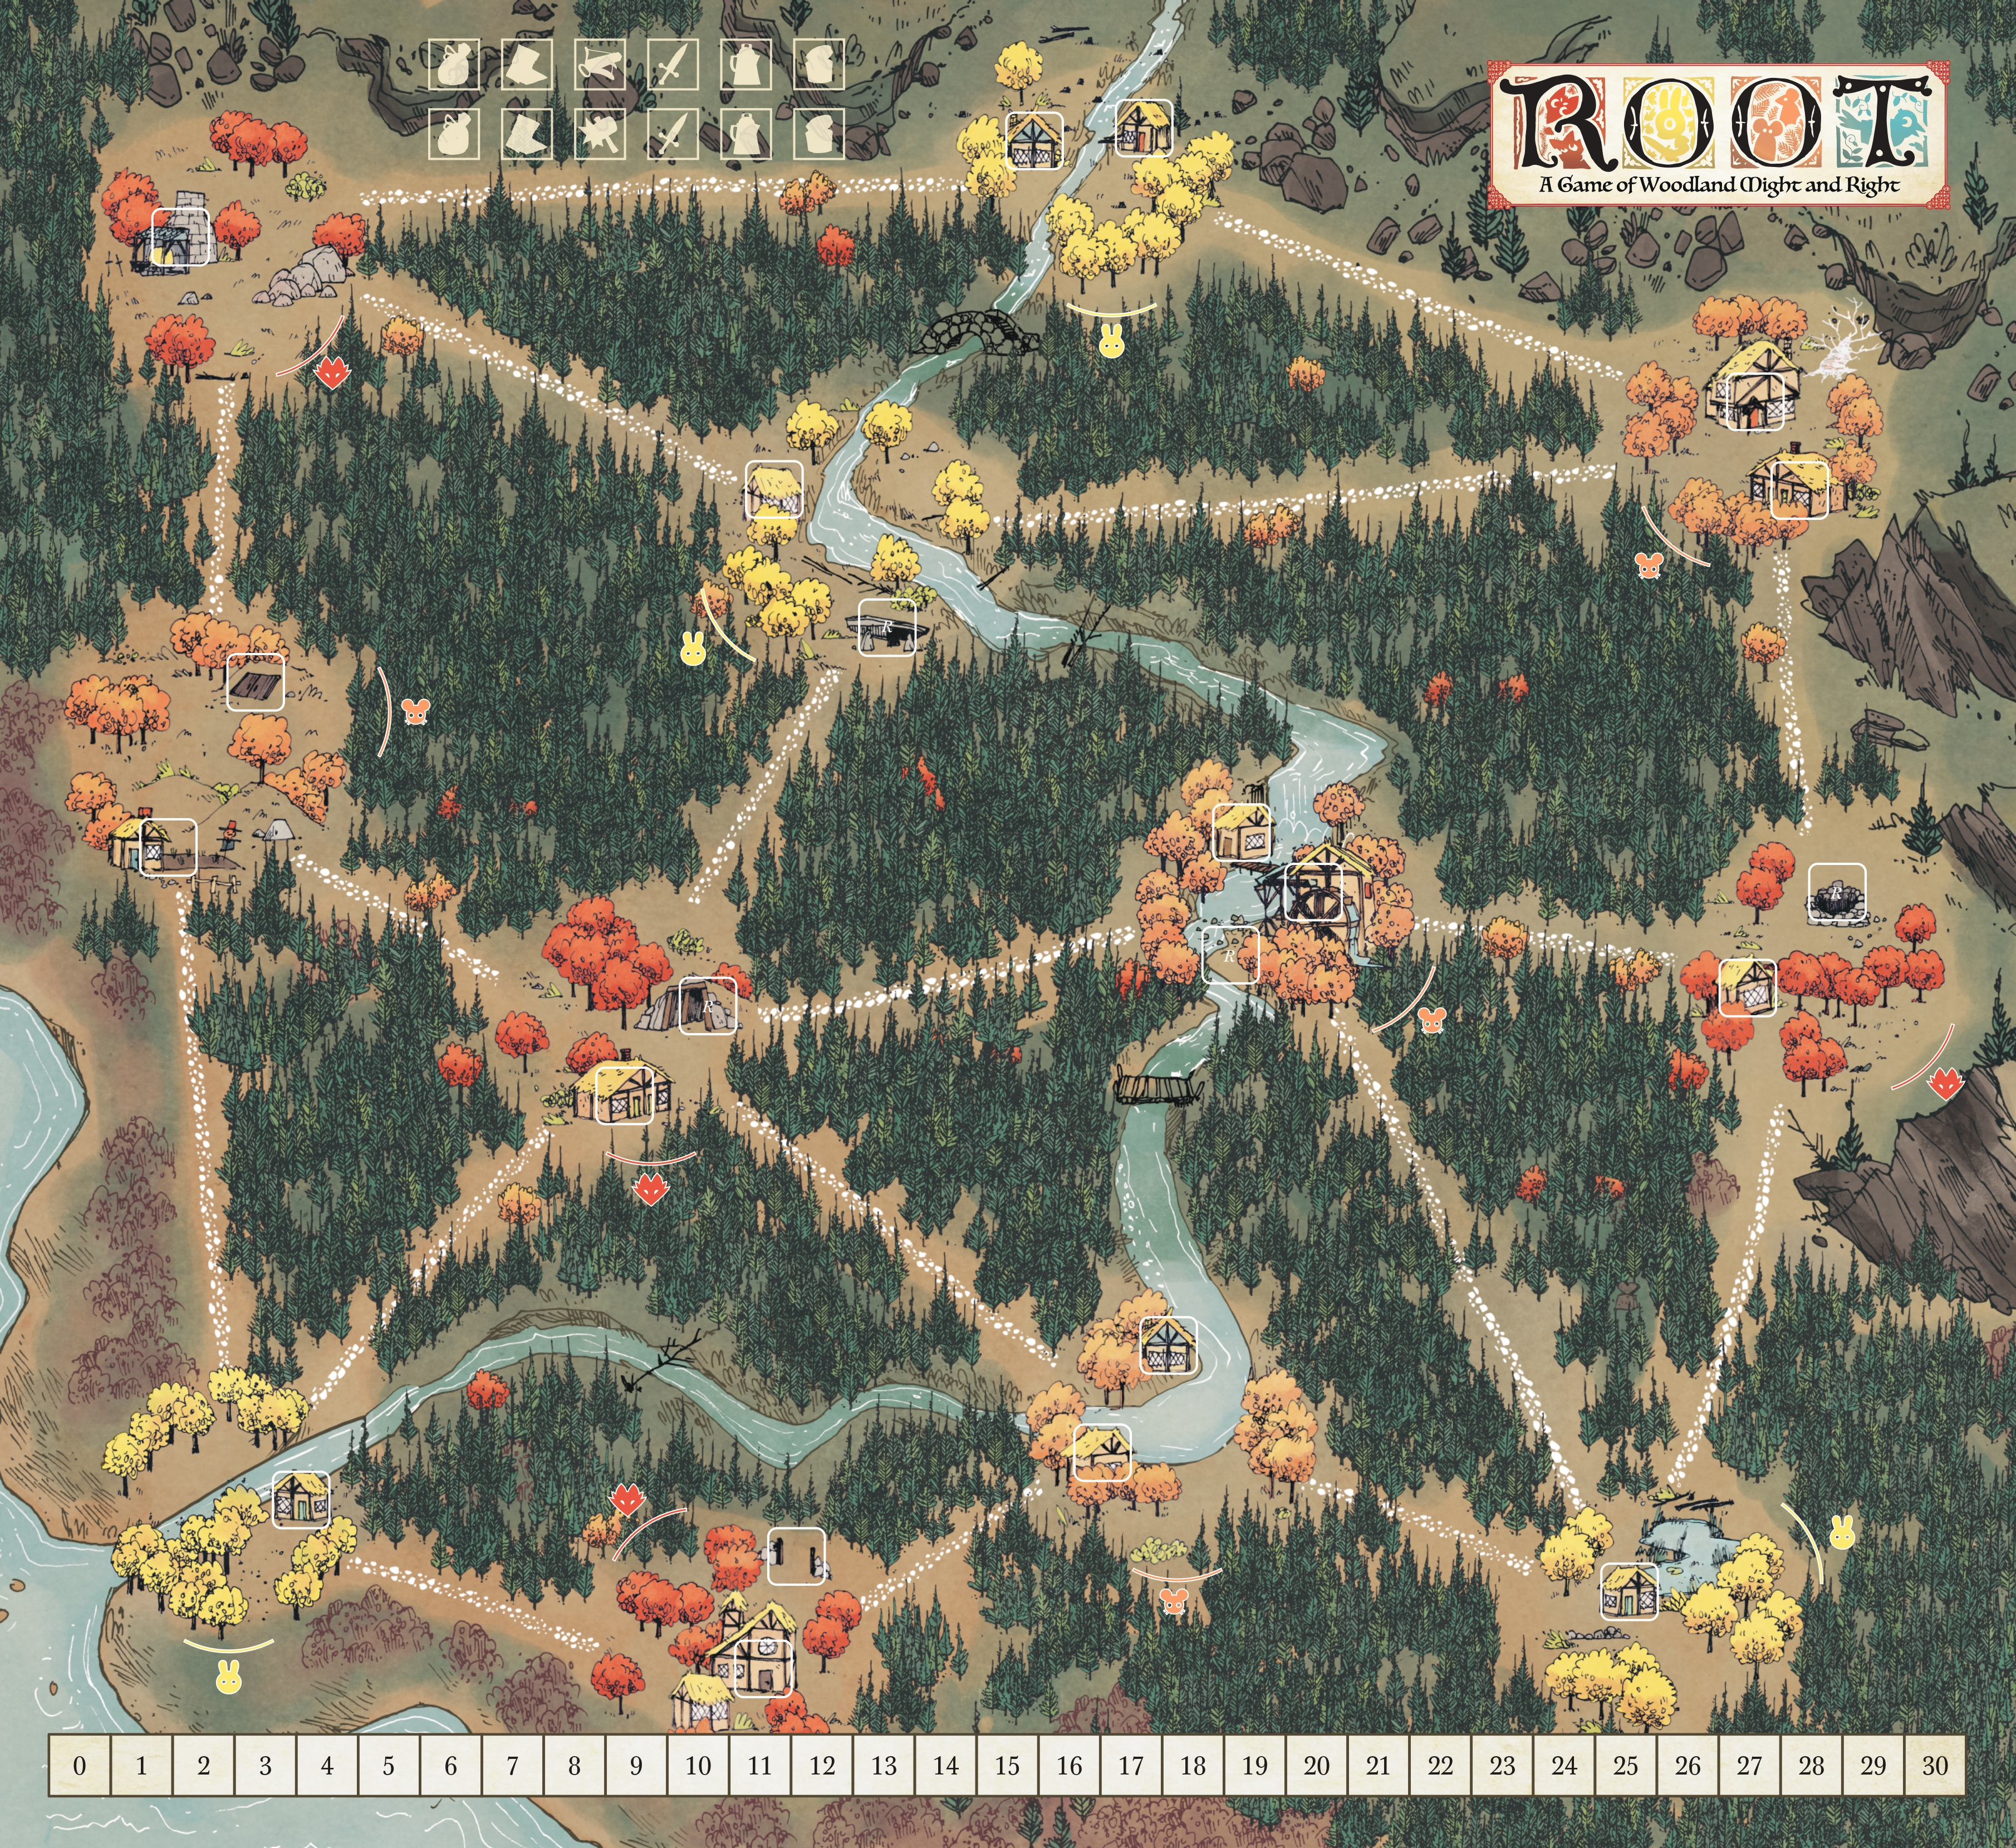
\includegraphics[width=14cm, height=14cm]{root_game_board.jpg}
  \end{center}
  \caption{Woodland, Root's game board}
  \label{fig:root-game-board}
\end{figure}

Each player will take his turn throughout three phases: birdsong, daylight, and evening. The player will be instructed on what he must do and what actions he can do in each phase. Also, each faction will have special abilities that can be used during their turn. Instructions and actions will vary from faction to faction, but there are actions that are shared by all factions, called key actions. There are three key actions:

\begin{enumerate}
  \item Move: Take any number of your warriors from one clearing and move them to one adjacent clearing.
  \item Craft: Using crafting pieces you have to craft a card from your hand. After crafting, gain benefits or effects on the crafted card.
  \item Battle: Choose a clearing where you have warriors as the clearing of battle. You are the attacker. Choose another player in the clearing of battle to be the defender. Roll two dice. The attacker deals hits equal to the higher roll, and the defender deals hits equal to the lower roll. Both players deal hits simultaneously and remove pieces equal to the number of hits they receive.
\end{enumerate}

Other than key actions, there will be some specific actions belonging to each faction. We will describe them in detail with an explanation of how each phase of each faction works in Table (2.1) and (2.2).

Some of the rules will not be explained here, as they are not crucial and essential. More rules can be found at \href{https://cdn.shopify.com/s/files/1/0106/0162/7706/files/Root_Base_Law_of_Root_June_10_2022.pdf?v=1661372308}{here}.

% \textit{[Add citation to Law of Root rule book/sheet/website]}  

\renewcommand{\arraystretch}{1.5}

\afterpage{
  \begin{landscape}
    \begin{table}
      \caption{\Marquise \ Flow}
      \label{tab:marquise-flow}
      \centering
      \begin{tabular}{|p{4cm}|p{12cm}|p{6cm}|} 
       \hline
        \multicolumn{3}{|c|}{\Marquise} \\
       \hline
       Birdsong & Daylight & Evening \\ 
       \hline
        \tabitem Place one wood token at each sawmill. 
      &\tabitem Craft any cards in your hand using workshops.
    
        \tabitem Take up to three of the following actions (plus one per bird suit card you spend): 
        
        \tabsubitem Battle

        \tabsubitem March: Takes two moves

        \tabsubitem Recruit: Place one warrior at each recruiter.

        \tabsubitem Build: Place one building in a clearing you rule by spending wood tokens equal to its cost.

        \tabsubitem Overwork: Spend a card to place one wood token at one sawmill in a clearing whose suit matches the card spent.
      &
        \tabitem Draw one card plus one card per draw bonus. (Discard down to five if you have more than five cards.)
      \\ 
       \hline
      \end{tabular}
    \end{table}
    
    \begin{table}
      \caption{\Eyrie \ Flow}
      \label{tab:eyrie-flow}
      \centering
      \begin{tabular}{|p{6cm}|p{11cm}|p{5cm}|} 
       \hline
        \multicolumn{3}{|c|}{\Eyrie} \\
       \hline
       Birdsong & Daylight & Evening \\ 
       \hline
       \tabitem If your hand is empty, draw 1 card.

       \tabitem Add one or two cards to the Decree.

       \tabitem If you have no roosts, place a roost and 3 warriors in the clearing with the fewest total pieces.
      & \tabitem Craft using roosts.

      \tabitem Resolve the Decree from left column to right, taking one action per card in a matching clearing

      \tabsubitem Recruit: Place warrior in a matching clearing

      \tabsubitem Move
      
      \tabsubitem Battle
      
      \tabsubitem Build: Place roost in a matching clearing you rule 
      &
      \tabitem Score victory point of rightmost empty space on the Roosts track.

      \tabitem Draw one card plus one card per draw bonus. (Discard down to five if you have more than five cards.)
      \\ 
       \hline
      \end{tabular}
    \end{table}
  \end{landscape}
}

\section{Second section}
Section 2 text.

\subsection{Subsection heading goes here}

Subsection 1 text

\subsubsection{Subsubsection 1 heading goes here}
Subsubsection 1 text

\subsubsection{Subsubsection 2 heading goes here}
Subsubsection 2 text

\section{Third section}
Section 3 text. The dielectric constant\index{dielectric constant}
at the air-metal interface determines
the resonance shift\index{resonance shift} as absorption or capture occurs
is shown in Equation~\eqref{eq:dielectric}:

\begin{equation}\label{eq:dielectric}
k_1=\frac{\omega}{c({1/\varepsilon_m + 1/\varepsilon_i})^{1/2}}=k_2=\frac{\omega
\sin(\theta)\varepsilon_\mathit{air}^{1/2}}{c}
\end{equation}

\noindent
where $\omega$ is the frequency of the plasmon, $c$ is the speed of
light, $\varepsilon_m$ is the dielectric constant of the metal,
$\varepsilon_i$ is the dielectric constant of neighboring insulator,
and $\varepsilon_\mathit{air}$ is the dielectric constant of air.

\section{About using figures in your report}

% define a command that produces some filler text, the lorem ipsum.
\newcommand{\loremipsum}{
  \textit{Lorem ipsum dolor sit amet, consectetur adipisicing elit, sed do
  eiusmod tempor incididunt ut labore et dolore magna aliqua. Ut enim ad
  minim veniam, quis nostrud exercitation ullamco laboris nisi ut
  aliquip ex ea commodo consequat. Duis aute irure dolor in
  reprehenderit in voluptate velit esse cillum dolore eu fugiat nulla
  pariatur. Excepteur sint occaecat cupidatat non proident, sunt in
  culpa qui officia deserunt mollit anim id est laborum.}\par}

\begin{figure}
  \centering

  \fbox{
     \parbox{.6\textwidth}{\loremipsum}
  }

  % To include an image in the figure, say myimage.pdf, you could use
  % the following code. Look up the documentation for the package
  % graphicx for more information.
  % \includegraphics[width=\textwidth]{myimage}

  \caption[Sample figure]{This figure is a sample containing \gls{lorem ipsum},
  showing you how you can include figures and glossary in your report.
  You can specify a shorter caption that will appear in the List of Figures.}
  \label{fig:sample-figure}
\end{figure}

Using \verb.\label. and \verb.\ref. commands allows us to refer to
figures easily. If we can refer to Figures
\ref{fig:walrus} and \ref{fig:sample-figure} by name in the {\LaTeX}
source code, then we will not need to update the code that refers to it
even if the placement or ordering of the figures changes.

\loremipsum\loremipsum

% This code demonstrates how to get a landscape table or figure. It
% uses the package lscape to turn everything but the page number into
% landscape orientation. Everything should be included within an
% \afterpage{ .... } to avoid causing a page break too early.
\afterpage{
  \begin{landscape}
  \begin{table}
    \caption{Sample landscape table}
    \label{tab:sample-table}

    \centering

    \begin{tabular}{c||c|c}
        Year & A & B \\
        \hline\hline
        1989 & 12 & 23 \\
        1990 & 4 & 9 \\
        1991 & 3 & 6 \\
    \end{tabular}
  \end{table}
  \end{landscape}
}

\loremipsum\loremipsum\loremipsum

\section{Overfull hbox}

When the \verb.semifinal. option is passed to the \verb.cpecmu. document class,
any line that is longer than the line width, i.e., an overfull hbox, will be
highlighted with a black solid rule:
\begin{center}
\begin{minipage}{2em}
juxtaposition
\end{minipage}
\end{center}

\section{\ifenglish%
\ifcpe CPE \else ISNE \fi knowledge used, applied, or integrated in this project
\else%
ความรู้ตามหลักสูตรซึ่งถูกนำมาใช้หรือบูรณาการในโครงงาน
\fi
}

อธิบายถึงความรู้ และแนวทางการนำความรู้ต่างๆ ที่ได้เรียนตามหลักสูตร ซึ่งถูกนำมาใช้ในโครงงาน

\section{\ifenglish%
Extracurricular knowledge used, applied, or integrated in this project
\else%
ความรู้นอกหลักสูตรซึ่งถูกนำมาใช้หรือบูรณาการในโครงงาน
\fi
}

อธิบายถึงความรู้ต่างๆ ที่เรียนรู้ด้วยตนเอง และแนวทางการนำความรู้เหล่านั้นมาใช้ในโครงงาน
